\documentclass{article}
\usepackage{ctex}
\usepackage{bm}
\usepackage[colorlinks, linkcolor=blue]{hyperref}
\usepackage{geometry}
\geometry{left=3cm, right=3cm, top=3cm, bottom=3cm}
\usepackage{amsmath}
\usepackage{amsthm}
\usepackage[T1]{fontenc}
\usepackage{xcolor}
\usepackage{lmodern}
\usepackage{listings}

\newtheorem{task}{问题}
\newtheorem*{proo}{证明}

\lstset{
	numbers=left, 
	numberstyle= \small, 
	keywordstyle= \color{ blue!70},
	commentstyle= \color{red!50!green!50!blue!50}, 
	frame=shadowbox, % 阴影效果
	showstringspaces = false,
	flexiblecolumns,                % 别问为什么,加上这个
	rulesepcolor= \color{ red!20!green!20!blue!20} ,
	escapeinside=``, % 英文分号中可写入中文
	breaklines=true,
	%xleftmargin=2em,xrightmargin=2em, aboveskip=1em,
	framexleftmargin=2.7em
}

\lstdefinestyle{Fortran}{
	language        =   [90]Fortran,
	basicstyle=\small\ttfamily
}

\title{作业四:插值算法}
\author{英才1701 赵鹏威 U201710152}

\begin{document}
	\maketitle
	\tableofcontents
	\newpage
	\section{引言}
	实验中得到的数据都是离散的,如果想知道测量位置以外的点的值,或者需要求积分导数,就需要有连续的函数形式. 一种做法是拟合,但是拟合得到的函数不一定经过给定的数据点. 如果要求函数必须经过给定的数据点,就需要使用插值算法.
	
	\section{问题描述}
	\begin{task}
		使用拉格朗日插值、牛顿插值和分段立方样条插值方法求下列数据点的插值函数
		\[
		y_i=\frac{1}{1+x_i^2},\quad x_i=-5+\frac{5-(-5)}{15}i,\quad i=0,1,\dots,15.
		\]
	\end{task}
	这个问题的数据点一共有16个,我们知道的是这16个点的x坐标和函数值y,不知道任何关于导数的信息. 这里需要说明的是,尽管问题的描述让我们感觉原函数是
	\[
	y=f(x)=\frac{1}{1+x^2},\quad x\in[-5,5],
	\]
	但是实际上我们并不知道原函数是什么,因为任何经过这16个点的函数都可能是原函数. 但是,作为对各种插值方法的分析,下面我们会将插值函数与$f(x)=1/(1+x^2)$画在同一张图里对比.
	
	\section{使用的误差分析公式}
	由于本次作业使用的误差估计式与课件上的有一些区别,因此单独作为一节来说明.
	\subsection{拉格朗日插值和牛顿插值}
	对于拉格朗日插值和牛顿插值,它们的真实误差(与真值的差)可以写成下面的形式
	\[
	R_{n+1}(x)=\frac{f^{(n+1)}(\xi)}{(n+1) !}\left(x-x_{0}\right) \cdots\left(x-x_{n}\right).
	\]
	但是这个公式需要知道原函数,实际不可操作. 因此有下面的做法. 假设有$n+1$个数据点,用前$n$个和后$n$个分别计算插值函数,近似认为$f^{(n+1)}(\xi)$相等,可以得到下面的误差估计式
	\[
	R_{n+1}(x)=\frac{x-x_{0}}{x_{0}-x_{n+1}}\left(L_{n}(x)-L_{n}^{\prime}(x)\right).
	\]
	上面是课件中给出的方法. 但是,这个误差估计式有一个缺点:当插值的数据点为偶数个并且关于y轴对称时,算出的误差恒为0. 下面来证明这一点,只要证明两次插值的函数完全一样即可.
	\begin{task}
		给定$2n$个插值数据点
		\[
		(-x_n,y_n),\;(-x_{n-1},y_{n-1}),\;\dots,\;(-x_2,y_2),\;(-x_1,y_1),\;(x_1,y_1),\;(x_2,y_2),\;\dots,(x_{n-1},y_{n-1}),\;(x_n,y_n)
		\]
		证明使用前$2n-1$个数据点
		\[
		(-x_n,y_n),\;(-x_{n-1},y_{n-1}),\;\dots,\;(-x_2,y_2),\;(-x_1,y_1),\;(x_1,y_1),\;(x_2,y_2),\;\dots,(x_{n-1},y_{n-1})
		\]
		得到的拉格朗日插值(或牛顿插值)函数$L_{-1}(x)$,与使用后$2n-1$个数据点
		\[
		(-x_{n-1},y_{n-1}),\;\dots,\;(-x_2,y_2),\;(-x_1,y_1),\;(x_1,y_1),\;(x_2,y_2),\;\dots,(x_{n-1},y_{n-1}),\;(x_n,y_n)
		\]
		得到的拉格朗日插值(或牛顿插值)函数$L_{+1}(x)$相等.
	\end{task}
	\begin{proo}
		由于拉格朗日插值和牛顿插值等价,下面使用牛顿插值来证明. 假设使用中间$2n-2$个数据点
		\[
		(-x_{n-1},y_{n-1}),\;\dots,\;(-x_2,y_2),\;(-x_1,y_1),\;(x_1,y_1),\;(x_2,y_2),\;\dots,(x_{n-1},y_{n-1})
		\]
		得到的插值函数为$L_0(x)$. 由于牛顿插值的特性,增加一个数据点再插值只需要在原来的插值函数上增加一项,可以知道
		\[
		L_{-1}(x)=L_0(x)+q_{-1}(x),\quad L_{+1}(x)=L_0(x)+q_{+1}(x)
		\]
		其中这些加上的项的表达式是可以算出的
		\[
		\begin{split}
		&q_{-1}(x)=f[-x_n,-x_{n-1},\dots,x_{n-1}]\Pi_{i=1}^{n-1}(x^2-x_i^2)\\
		&q_{+1}(x)=f[-x_{n-1},\dots,\;\,x_{n-1},\;\,x_n]\Pi_{i=1}^{n-1}(x^2-x_i^2)
		\end{split}
		\]
		那么只要证明 $f[-x_n,-x_{n-1},\dots,x_{n-1}]=f[-x_{n-1},\dots,\;\,x_{n-1},\;\,x_n]$. 可以发现,只要将等号左边的差商括号里的每一项取相反数,就得到了等号右边的差商. 利用偶函数差商的性质:
		\[
		f[-x_1,\dots,-x_n]=(-1)^{n+1}f[x_1,\dots,x_n],
		\]
		立即可以证明$f[-x_n,-x_{n-1},\dots,x_{n-1}]=f[-x_{n-1},\dots,\;\,x_{n-1},\;\,x_n]$. 因此$L_{-1}(x)=L_{+1}(x)$. 证毕.
	\end{proo}
	
	不幸的是,这次作业给出的数据点刚好是关于y轴对称的,因此我们需要换一种误差估计公式. 比如有$n$个数据点,用前$n-2$个点插值得到$L(x)$,用后$n-2$个点插值得到$L'(x)$,可以推导下面的误差估计式
	\[
	R=f(x)-\frac{L(x)+L'(x)}{2}=\frac{(x-x_n)(x-x_{n-1})+(x-x_1)(x-x_2)}{(x-x_n)(x-x_{n-1})-(x-x_1)(x-x_2)}\frac{L(x)-L'(x)}{2}
	\]
	下面在估计拉格朗日插值和牛顿插值的误差时均使用这个误差估计式.
	\subsection{分段立方样条插值}
	由于分段立方样条插值的每一段都是一个两点三次 Hermit 插值. Hermit 插值的误差估计式同样含有原函数的导数项,但是如果按照上面的方法尝试用两个插值来消去这个导数项,就会因为插值的点只有一个而产生较大的误差. 另外由于没有找到较好的误差估计方法,本次作业的分段立方样条插值将使用真实误差,其中原函数认为是
	\[
	f(x)=\frac{1}{1+x^2}.
	\]
	
	\section{程序实现}
	所有的插值算法都用 function 实现,接受数据点参数 sample 和一个 x 值,函数用指定的插值算法计算出插值函数在 x 点的值. 另外,函数返回的类型是另外定义的 result 类型,可以同时储存值和误差. 函数还接受一个参数,require\_error,如果这个参数为真,那么会计算误差,否则不会. require\_error 默认为真. 完整代码见附录.
	\subsection{拉格朗日插值}
	拉格朗日插值,流程图见图\ref{fig:lagrange},代码见 Listing \ref{lagrange.f90}.
	\begin{figure}[h!tb]
		\centering
		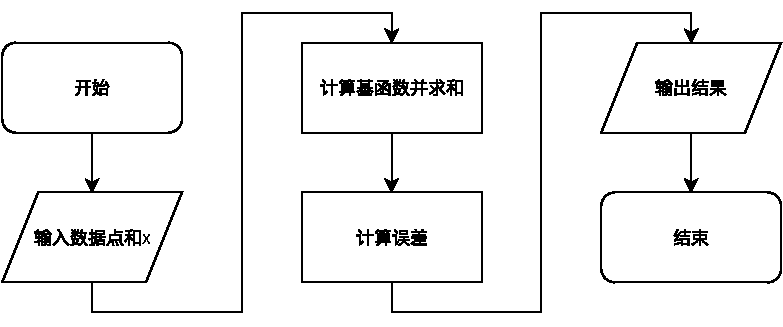
\includegraphics[width=0.8\textwidth]{./utils/lagrange.pdf}
		\caption{ 拉格朗日插值流程图\label{fig:lagrange}}
	\end{figure}
	\lstinputlisting[
	style = Fortran,
	caption     =   {\bf 拉格朗日插值},
	label       =   {lagrange.f90}
	]{./utils/snips/lagrange.f90}
	\subsection{牛顿插值}
	牛顿插值需要用到差商,我选择的是写一个计算差商的函数,每次需要的时候就调用这个函数. 虽然这样做会降低效率,但是程序看起来会更简单,并且只需要在拉格朗日插值代码的基础上稍作一些修改即可. 差商用递归实现,代码见 Listing \ref{diff_quot.f90}. 牛顿插值的流程图见\ref{fig:newton},代码见 Listing \ref{newton.f90}.
	\begin{figure}[h!tb]
		\centering
		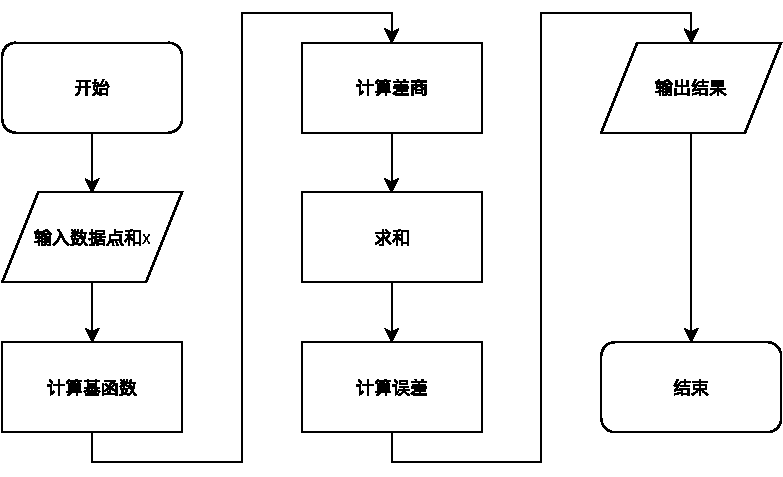
\includegraphics[width=0.8\textwidth]{./utils/newton.pdf}
		\caption{ 牛顿插值流程图\label{fig:newton}}
	\end{figure}
	\lstinputlisting[
	style = Fortran,
	caption     =   {\bf 差商},
	label       =   {diff_quot.f90}
	]{./utils/snips/diff_quot.f90}
	\lstinputlisting[
	style = Fortran,
	caption     =   {\bf 牛顿插值},
	label       =   {newton.f90}
	]{./utils/snips/newton.f90}
	\subsection{分段立方样条插值}
	这里使用的边界条件是两端的一阶导为0,因此需要解三转角方程,可以使用追赶法. 追赶法的程序见 Listing \ref{chasing_method.f90}. 分段立方样条插值流程图见图\ref{fig:cubic_spline},代码见 Listing \ref{cubic_spline.f90}. 
	\begin{figure}[h!tb]
		\centering
		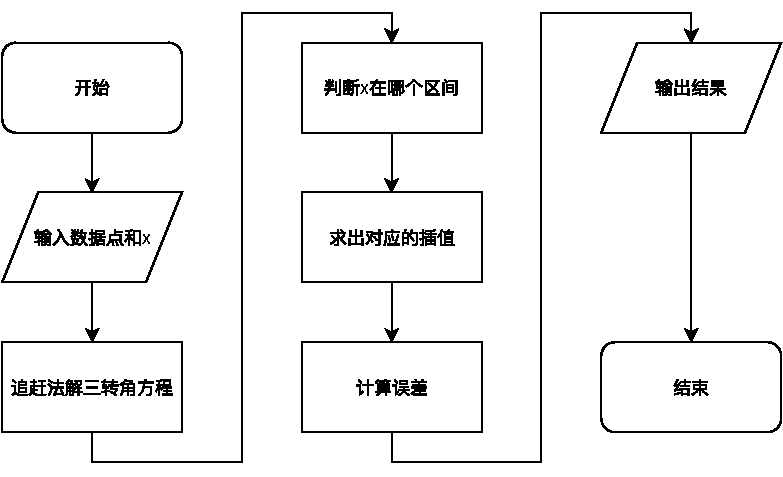
\includegraphics[width=0.8\textwidth]{./utils/cubic_spline.pdf}
		\caption{ 分段立方样条插值流程图\label{fig:cubic_spline}}
	\end{figure}
	\lstinputlisting[
	style = Fortran,
	caption     =   {\bf 追赶法},
	label       =   {chasing_method.f90}
	]{./utils/snips/chasing_method.f90}
	\lstinputlisting[
	style = Fortran,
	caption     =   {\bf 分段立方样条插值},
	label       =   {cubic_spline.f90}
	]{./utils/snips/cubic_spline.f90}
	
	\section{插值结果}
	下面的结果是由问题给出的16个数据点插值,并在$[-5,5]$的区间内选取10000个点绘制的图像,结果见图\ref{fig:result},上面的三个图是插值曲线,下面的三个图是画出误差棒的插值曲线,由于点取的很密,所以误差棒看起来是连续的,这样可以反应整体的误差分布情况. 拉格朗日插值的结果如图\ref{fig:result}左图所示. 可见出现了龙格现象,在两端的插值出现很大的误差,而在区间中心误差较小. 牛顿插值结果见图\ref{fig:result}中图所示,可见插值结果与拉格朗日插值完全一样. 分段立方样条插值结果如图\ref{fig:result}右图所示,可见两端的误差较小,中间的误差较大. 整体来讲,这三种方法中,分段立方样条插值的结果抖动更小,并且与原函数更接近. 但是就实际问题来讲,并没有理由说明抖动更小的结果就更接近真实值,因为真实值很多情况下是不可知的.
	\begin{figure}[h!tb]
		\centering
		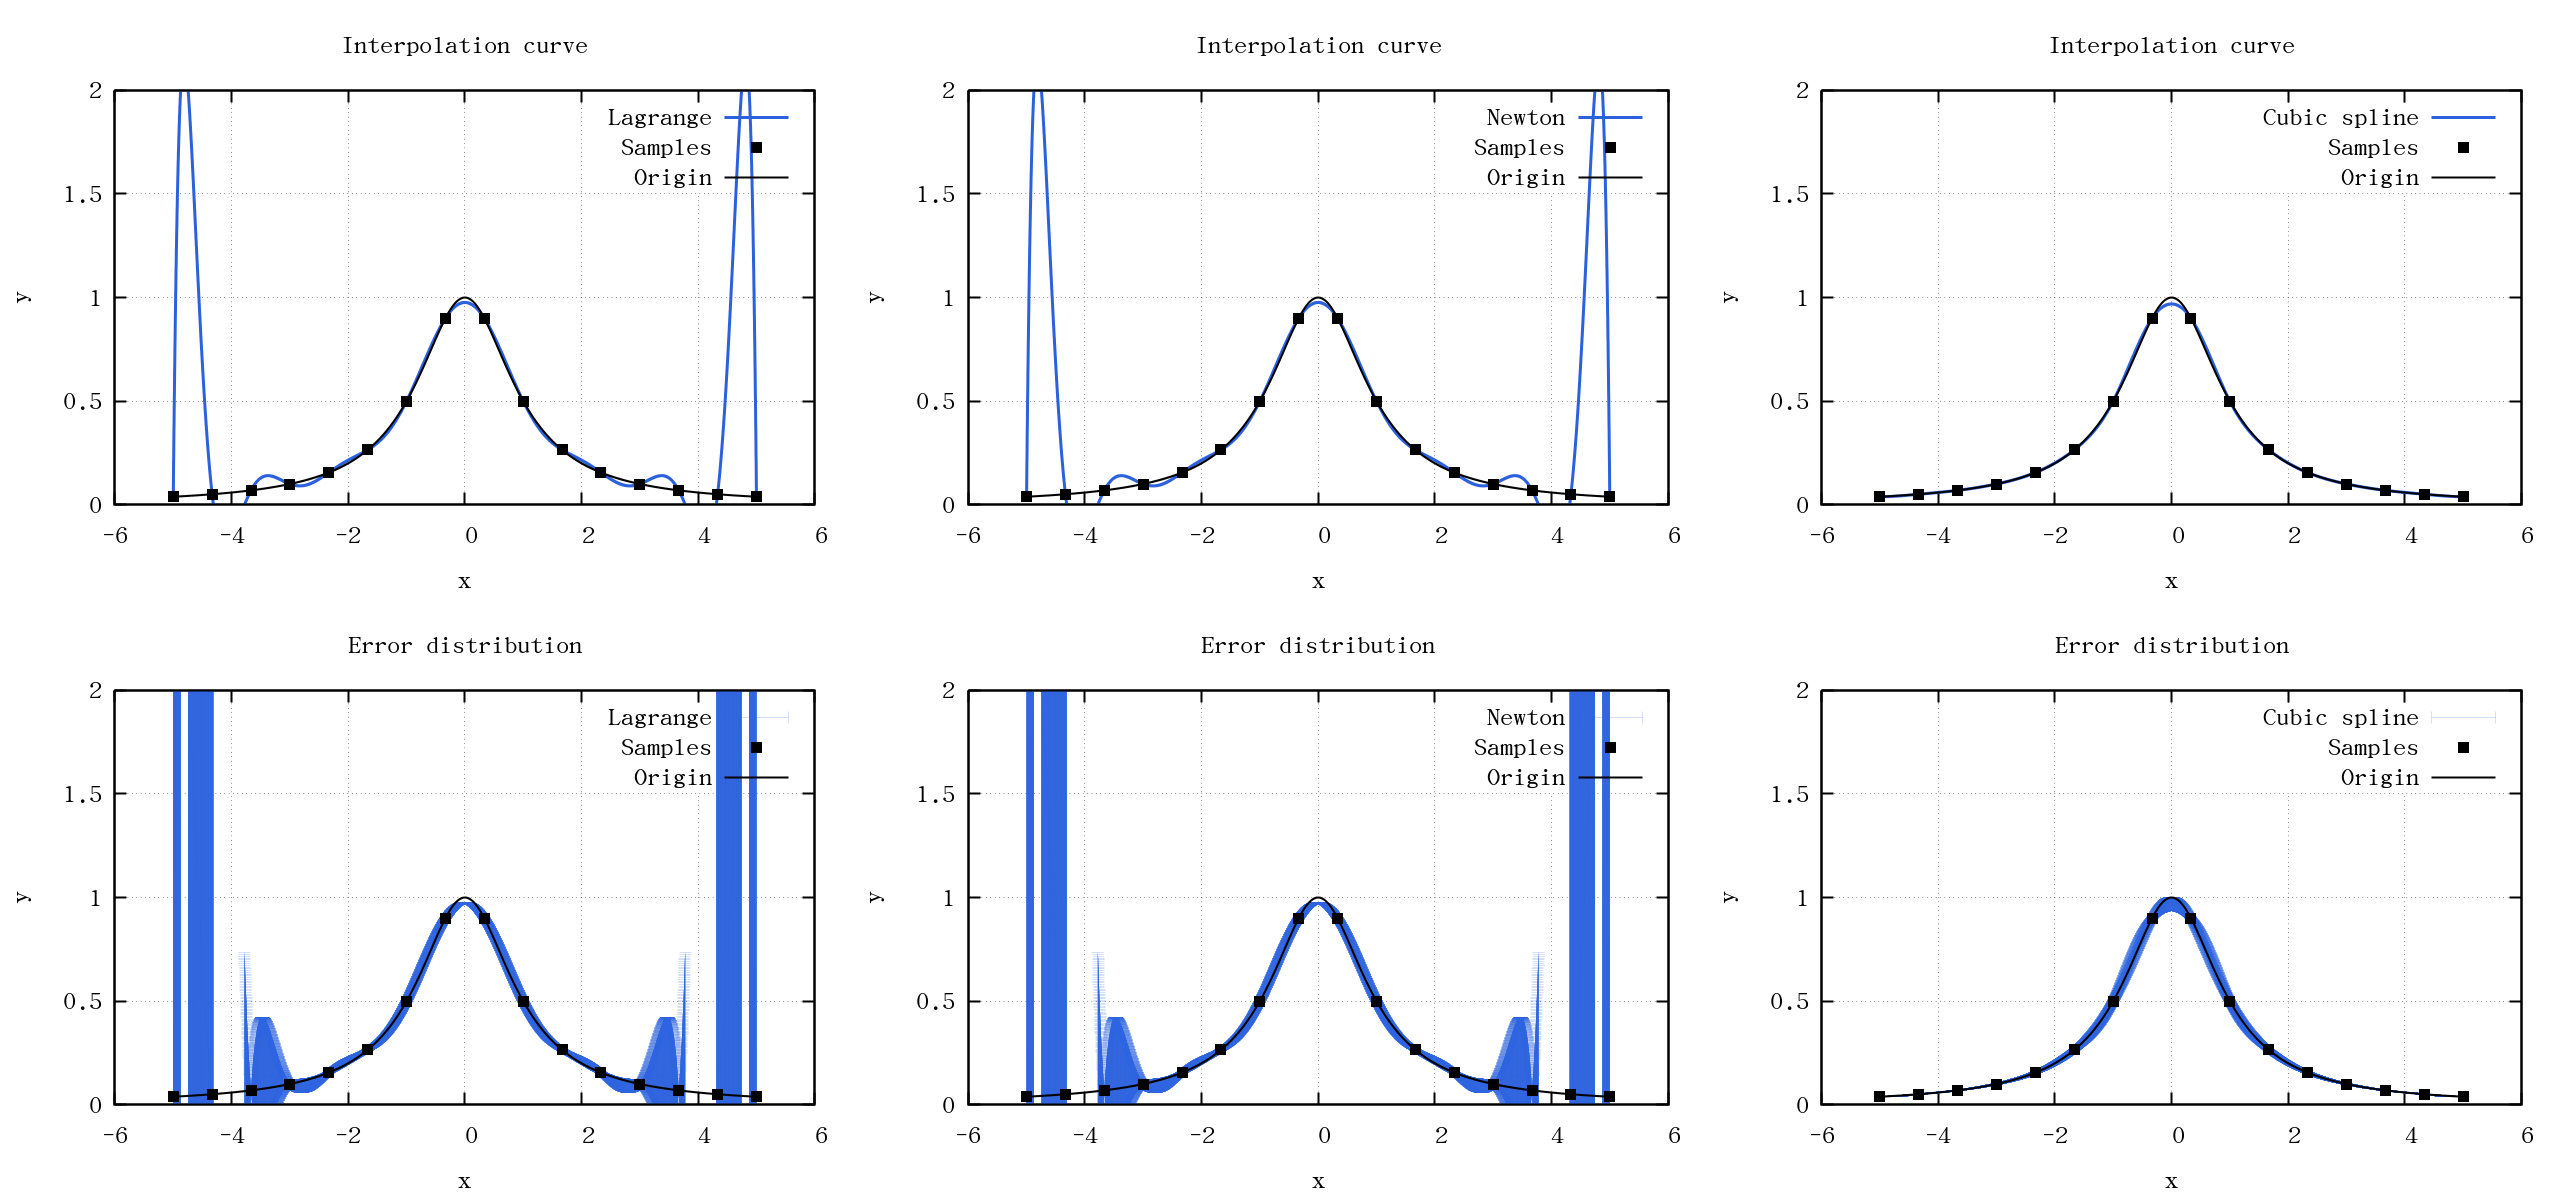
\includegraphics[width=1.0\textwidth]{./utils/result.png}
		\caption{ 三种方法的插值结果\label{fig:result}}
	\end{figure}

	\newpage
	\section*{附录}
	代码可在\url{https://github.com/ZipWin/computational_physics/tree/master/assignments/assignment4}找到.
	\lstinputlisting[
	style = Fortran,
	caption     =   {\bf interpolation.f90},
	label       =   {interpolation.f90}
	]{./utils/interpolation.f90}
	
\end{document}